\chapter{The Treasure}

When Dantès returned next morning to the chamber of his companion in
captivity, he found Faria seated and looking composed. In the ray of
light which entered by the narrow window of his cell, he held open in
his left hand, of which alone, it will be recollected, he retained the
use, a sheet of paper, which, from being constantly rolled into a small
compass, had the form of a cylinder, and was not easily kept open. He
did not speak, but showed the paper to Dantès.

“What is that?” he inquired.

“Look at it,” said the abbé with a smile.

“I have looked at it with all possible attention,” said Dantès, “and I
only see a half-burnt paper, on which are traces of Gothic characters
inscribed with a peculiar kind of ink.”

“This paper, my friend,” said Faria, “I may now avow to you, since I
have the proof of your fidelity—this paper is my treasure, of which,
from this day forth, one-half belongs to you.”

The sweat started forth on Dantès’ brow. Until this day and for how
long a time!—he had refrained from talking of the treasure, which had
brought upon the abbé the accusation of madness. With his instinctive
delicacy Edmond had preferred avoiding any touch on this painful chord,
and Faria had been equally silent. He had taken the silence of the old
man for a return to reason; and now these few words uttered by Faria,
after so painful a crisis, seemed to indicate a serious relapse into
mental alienation.

“Your treasure?” stammered Dantès. Faria smiled.

“Yes,” said he. “You have, indeed, a noble nature, Edmond, and I see by
your paleness and agitation what is passing in your heart at this
moment. No, be assured, I am not mad. This treasure exists, Dantès, and
if I have not been allowed to possess it, you will. Yes—you. No one
would listen or believe me, because everyone thought me mad; but you,
who must know that I am not, listen to me, and believe me so afterwards
if you will.”

“Alas,” murmured Edmond to himself, “this is a terrible relapse! There
was only this blow wanting.” Then he said aloud, “My dear friend, your
attack has, perhaps, fatigued you; had you not better repose awhile?
Tomorrow, if you will, I will hear your narrative; but today I wish to
nurse you carefully. Besides,” he said, “a treasure is not a thing we
need hurry about.”

“On the contrary, it is a matter of the utmost importance, Edmond!”
replied the old man. “Who knows if tomorrow, or the next day after, the
third attack may not come on? and then must not all be over? Yes,
indeed, I have often thought with a bitter joy that these riches, which
would make the wealth of a dozen families, will be forever lost to
those men who persecute me. This idea was one of vengeance to me, and I
tasted it slowly in the night of my dungeon and the despair of my
captivity. But now I have forgiven the world for the love of you; now
that I see you, young and with a promising future,—now that I think of
all that may result to you in the good fortune of such a disclosure, I
shudder at any delay, and tremble lest I should not assure to one as
worthy as yourself the possession of so vast an amount of hidden
wealth.”

Edmond turned away his head with a sigh.

“You persist in your incredulity, Edmond,” continued Faria. “My words
have not convinced you. I see you require proofs. Well, then, read this
paper, which I have never shown to anyone.”

“Tomorrow, my dear friend,” said Edmond, desirous of not yielding to
the old man’s madness. “I thought it was understood that we should not
talk of that until tomorrow.”

“Then we will not talk of it until tomorrow; but read this paper
today.”

“I will not irritate him,” thought Edmond, and taking the paper, of
which half was wanting,—having been burnt, no doubt, by some
accident,—he read:

\vskip \onelineskip

\begin{quote}
{\small“this treasure, which may amount to two...

of Roman crowns in the most distant a...

of the second opening wh...

declare to belong to him alo...

heir.

\hspace{6em}“25th April, 149’”}
\end{quote}

\vskip \onelineskip

“Well!” said Faria, when the young man had finished reading it.

“Why,” replied Dantès, “I see nothing but broken lines and unconnected
words, which are rendered illegible by fire.”

“Yes, to you, my friend, who read them for the first time; but not for
me, who have grown pale over them by many nights’ study, and have
reconstructed every phrase, completed every thought.”

“And do you believe you have discovered the hidden meaning?”

“I am sure I have, and you shall judge for yourself; but first listen
to the history of this paper.”

“Silence!” exclaimed Dantès. “Steps approach—I go—adieu!”

And Dantès, happy to escape the history and explanation which would be
sure to confirm his belief in his friend’s mental instability, glided
like a snake along the narrow passage; while Faria, restored by his
alarm to a certain amount of activity, pushed the stone into place with
his foot, and covered it with a mat in order the more effectually to
avoid discovery.

It was the governor, who, hearing of Faria’s illness from the jailer,
had come in person to see him.

Faria sat up to receive him, avoiding all gestures in order that he
might conceal from the governor the paralysis that had already half
stricken him with death. His fear was lest the governor, touched with
pity, might order him to be removed to better quarters, and thus
separate him from his young companion. But fortunately this was not the
case, and the governor left him, convinced that the poor madman, for
whom in his heart he felt a kind of affection, was only troubled with a
slight indisposition.

During this time, Edmond, seated on his bed with his head in his hands,
tried to collect his scattered thoughts. Faria, since their first
acquaintance, had been on all points so rational and logical, so
wonderfully sagacious, in fact, that he could not understand how so
much wisdom on all points could be allied with madness. Was Faria
deceived as to his treasure, or was all the world deceived as to Faria?

Dantès remained in his cell all day, not daring to return to his
friend, thinking thus to defer the moment when he should be convinced,
once for all, that the abbé was mad—such a conviction would be so
terrible!

But, towards the evening after the hour for the customary visit had
gone by, Faria, not seeing the young man appear, tried to move and get
over the distance which separated them. Edmond shuddered when he heard
the painful efforts which the old man made to drag himself along; his
leg was inert, and he could no longer make use of one arm. Edmond was
obliged to assist him, for otherwise he would not have been able to
enter by the small aperture which led to Dantès’ chamber.

“Here I am, pursuing you remorselessly,” he said with a benignant
smile. “You thought to escape my munificence, but it is in vain. Listen
to me.”

Edmond saw there was no escape, and placing the old man on his bed, he
seated himself on the stool beside him.

“You know,” said the abbé, “that I was the secretary and intimate
friend of Cardinal Spada, the last of the princes of that name. I owe
to this worthy lord all the happiness I ever knew. He was not rich,
although the wealth of his family had passed into a proverb, and I
heard the phrase very often, ‘As rich as a Spada.’ But he, like public
rumor, lived on this reputation for wealth; his palace was my paradise.
I was tutor to his nephews, who are dead; and when he was alone in the
world, I tried by absolute devotion to his will, to make up to him all
he had done for me during ten years of unremitting kindness. The
cardinal’s house had no secrets for me. I had often seen my noble
patron annotating ancient volumes, and eagerly searching amongst dusty
family manuscripts. One day when I was reproaching him for his
unavailing searches, and deploring the prostration of mind that
followed them, he looked at me, and, smiling bitterly, opened a volume
relating to the History of the City of Rome. There, in the twentieth
chapter of the Life of Pope Alexander VI., were the following lines,
which I can never forget:—

“‘The great wars of Romagna had ended; Cæsar Borgia, who had completed
his conquest, had need of money to purchase all Italy. The pope had
also need of money to bring matters to an end with Louis XII. King of
France, who was formidable still in spite of his recent reverses; and
it was necessary, therefore, to have recourse to some profitable
scheme, which was a matter of great difficulty in the impoverished
condition of exhausted Italy. His holiness had an idea. He determined
to make two cardinals.’

“By choosing two of the greatest personages of Rome, especially rich
men—\textit{this} was the return the Holy Father looked for. In the first
place, he could sell the great appointments and splendid offices which
the cardinals already held; and then he had the two hats to sell
besides. There was a third point in view, which will appear hereafter.

“The pope and Cæsar Borgia first found the two future cardinals; they
were Giovanni Rospigliosi, who held four of the highest dignities of
the Holy See, and Cæsar Spada, one of the noblest and richest of the
Roman nobility; both felt the high honor of such a favor from the pope.
They were ambitious, and Cæsar Borgia soon found purchasers for their
appointments. The result was, that Rospigliosi and Spada paid for being
cardinals, and eight other persons paid for the offices the cardinals
held before their elevation, and thus eight hundred thousand crowns
entered into the coffers of the speculators.

\begin{figure}[ht]
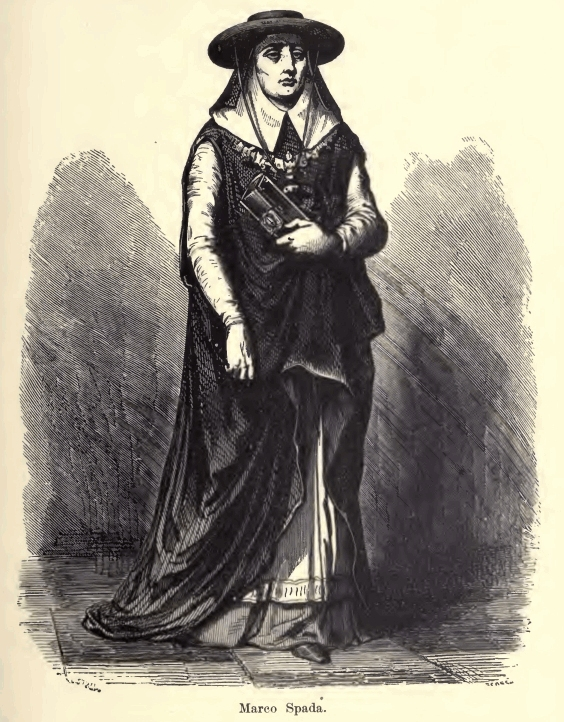
\includegraphics[width=\textwidth]{0239m.jpg}
\end{figure}

“It is time now to proceed to the last part of the speculation. The
pope heaped attentions upon Rospigliosi and Spada, conferred upon them
the insignia of the cardinalate, and induced them to arrange their
affairs and take up their residence at Rome. Then the pope and Cæsar
Borgia invited the two cardinals to dinner. This was a matter of
dispute between the Holy Father and his son. Cæsar thought they could
make use of one of the means which he always had ready for his friends,
that is to say, in the first place, the famous key which was given to
certain persons with the request that they go and open a designated
cupboard. This key was furnished with a small iron point,—a negligence
on the part of the locksmith. When this was pressed to effect the
opening of the cupboard, of which the lock was difficult, the person
was pricked by this small point, and died next day. Then there was the
ring with the lion’s head, which Cæsar wore when he wanted to greet his
friends with a clasp of the hand. The lion bit the hand thus favored,
and at the end of twenty-four hours, the bite was mortal.

“Cæsar proposed to his father, that they should either ask the
cardinals to open the cupboard, or shake hands with them; but Alexander
VI. replied: ‘Now as to the worthy cardinals, Spada and Rospigliosi,
let us ask both of them to dinner, something tells me that we shall get
that money back. Besides, you forget, Cæsar, an indigestion declares
itself immediately, while a prick or a bite occasions a delay of a day
or two.’ Cæsar gave way before such cogent reasoning, and the cardinals
were consequently invited to dinner.

“The table was laid in a vineyard belonging to the pope, near San
Pierdarena, a charming retreat which the cardinals knew very well by
report. Rospigliosi, quite set up with his new dignities, went with a
good appetite and his most ingratiating manner. Spada, a prudent man,
and greatly attached to his only nephew, a young captain of the highest
promise, took paper and pen, and made his will. He then sent word to
his nephew to wait for him near the vineyard; but it appeared the
servant did not find him.

“Spada knew what these invitations meant; since Christianity, so
eminently civilizing, had made progress in Rome, it was no longer a
centurion who came from the tyrant with a message, ‘Cæsar wills that
you die.’ but it was a legate \textit{à latere}, who came with a smile on his
lips to say from the pope, ‘His holiness requests you to dine with
him.’

“Spada set out about two o’clock to San Pierdarena. The pope awaited
him. The first sight that attracted the eyes of Spada was that of his
nephew, in full costume, and Cæsar Borgia paying him most marked
attentions. Spada turned pale, as Cæsar looked at him with an ironical
air, which proved that he had anticipated all, and that the snare was
well spread.

“They began dinner and Spada was only able to inquire of his nephew if
he had received his message. The nephew replied no; perfectly
comprehending the meaning of the question. It was too late, for he had
already drunk a glass of excellent wine, placed for him expressly by
the pope’s butler. Spada at the same moment saw another bottle approach
him, which he was pressed to taste. An hour afterwards a physician
declared they were both poisoned through eating mushrooms. Spada died
on the threshold of the vineyard; the nephew expired at his own door,
making signs which his wife could not comprehend.

“Then Cæsar and the pope hastened to lay hands on the heritage, under
pretense of seeking for the papers of the dead man. But the inheritance
consisted in this only, a scrap of paper on which Spada had written:—‘I
bequeath to my beloved nephew my coffers, my books, and, amongst
others, my breviary with the gold corners, which I beg he will preserve
in remembrance of his affectionate uncle.’

“The heirs sought everywhere, admired the breviary, laid hands on the
furniture, and were greatly astonished that Spada, the rich man, was
really the most miserable of uncles—no treasures—unless they were those
of science, contained in the library and laboratories. That was all.
Cæsar and his father searched, examined, scrutinized, but found
nothing, or at least very little; not exceeding a few thousand crowns
in plate, and about the same in ready money; but the nephew had time to
say to his wife before he expired: ‘Look well among my uncle’s papers;
there is a will.’

“They sought even more thoroughly than the august heirs had done, but
it was fruitless. There were two palaces and a vineyard behind the
Palatine Hill; but in these days landed property had not much value,
and the two palaces and the vineyard remained to the family since they
were beneath the rapacity of the pope and his son. Months and years
rolled on. Alexander VI. died, poisoned,—you know by what mistake.
Cæsar, poisoned at the same time, escaped by shedding his skin like a
snake; but the new skin was spotted by the poison till it looked like a
tiger’s. Then, compelled to quit Rome, he went and got himself
obscurely killed in a night skirmish, scarcely noticed in history.

“After the pope’s death and his son’s exile, it was supposed that the
Spada family would resume the splendid position they had held before
the cardinal’s time; but this was not the case. The Spadas remained in
doubtful ease, a mystery hung over this dark affair, and the public
rumor was, that Cæsar, a better politician than his father, had carried
off from the pope the fortune of the two cardinals. I say the two,
because Cardinal Rospigliosi, who had not taken any precaution, was
completely despoiled.

“Up to this point,” said Faria, interrupting the thread of his
narrative, “this seems to you very meaningless, no doubt, eh?”

“Oh, my friend,” cried Dantès, “on the contrary, it seems as if I were
reading a most interesting narrative; go on, I beg of you.”

“I will. The family began to get accustomed to their obscurity. Years
rolled on, and amongst the descendants some were soldiers, others
diplomatists; some churchmen, some bankers; some grew rich, and some
were ruined. I come now to the last of the family, whose secretary I
was—the Count of Spada. I had often heard him complain of the
disproportion of his rank with his fortune; and I advised him to invest
all he had in an annuity. He did so, and thus doubled his income. The
celebrated breviary remained in the family, and was in the count’s
possession. It had been handed down from father to son; for the
singular clause of the only will that had been found, had caused it to
be regarded as a genuine relic, preserved in the family with
superstitious veneration. It was an illuminated book, with beautiful
Gothic characters, and so weighty with gold, that a servant always
carried it before the cardinal on days of great solemnity.

“At the sight of papers of all sorts,—titles, contracts, parchments,
which were kept in the archives of the family, all descending from the
poisoned cardinal, I in my turn examined the immense bundles of
documents, like twenty servitors, stewards, secretaries before me; but
in spite of the most exhaustive researches, I found—nothing. Yet I had
read, I had even written a precise history of the Borgia family, for
the sole purpose of assuring myself whether any increase of fortune had
occurred to them on the death of the Cardinal Cæsar Spada; but could
only trace the acquisition of the property of the Cardinal Rospigliosi,
his companion in misfortune.

“I was then almost assured that the inheritance had neither profited
the Borgias nor the family, but had remained unpossessed like the
treasures of the Arabian Nights, which slept in the bosom of the earth
under the eyes of the genie. I searched, ransacked, counted, calculated
a thousand and a thousand times the income and expenditure of the
family for three hundred years. It was useless. I remained in my
ignorance, and the Count of Spada in his poverty.

“My patron died. He had reserved from his annuity his family papers,
his library, composed of five thousand volumes, and his famous
breviary. All these he bequeathed to me, with a thousand Roman crowns,
which he had in ready money, on condition that I would have anniversary
masses said for the repose of his soul, and that I would draw up a
genealogical tree and history of his house. All this I did
scrupulously. Be easy, my dear Edmond, we are near the conclusion.

“In 1807, a month before I was arrested, and a fortnight after the
death of the Count of Spada, on the 25th of December (you will see
presently how the date became fixed in my memory), I was reading, for
the thousandth time, the papers I was arranging, for the palace was
sold to a stranger, and I was going to leave Rome and settle at
Florence, intending to take with me twelve thousand francs I possessed,
my library, and the famous breviary, when, tired with my constant labor
at the same thing, and overcome by a heavy dinner I had eaten, my head
dropped on my hands, and I fell asleep about three o’clock in the
afternoon.

\begin{figure}[ht]
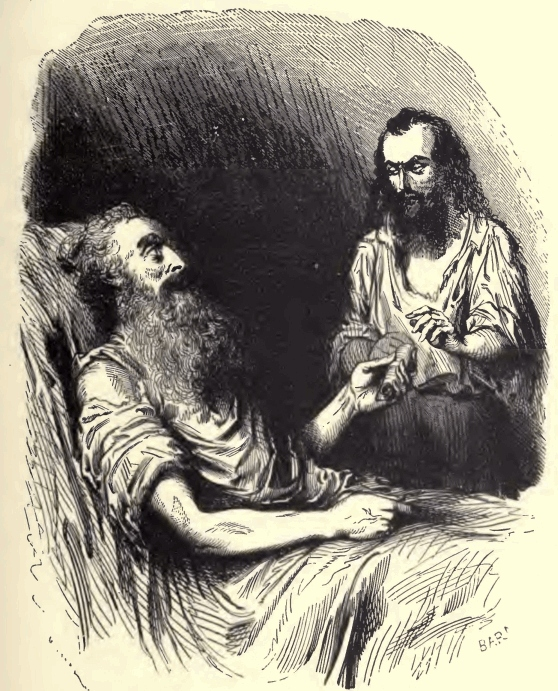
\includegraphics[width=\textwidth]{0243m.jpg}
\end{figure}

“I awoke as the clock was striking six. I raised my head; I was in
utter darkness. I rang for a light, but, as no one came, I determined
to find one for myself. It was indeed but anticipating the simple
manners which I should soon be under the necessity of adopting. I took
a wax-candle in one hand, and with the other groped about for a piece
of paper (my match-box being empty), with which I proposed to get a
light from the small flame still playing on the embers. Fearing,
however, to make use of any valuable piece of paper, I hesitated for a
moment, then recollected that I had seen in the famous breviary, which
was on the table beside me, an old paper quite yellow with age, and
which had served as a marker for centuries, kept there by the request
of the heirs. I felt for it, found it, twisted it up together, and
putting it into the expiring flame, set light to it.

“But beneath my fingers, as if by magic, in proportion as the fire
ascended, I saw yellowish characters appear on the paper. I grasped it
in my hand, put out the flame as quickly as I could, lighted my taper
in the fire itself, and opened the crumpled paper with inexpressible
emotion, recognizing, when I had done so, that these characters had
been traced in mysterious and sympathetic ink, only appearing when
exposed to the fire; nearly one-third of the paper had been consumed by
the flame. It was that paper you read this morning; read it again,
Dantès, and then I will complete for you the incomplete words and
unconnected sense.”

Faria, with an air of triumph, offered the paper to Dantès, who this
time read the following words, traced with an ink of a reddish color
resembling rust:

\vskip \onelineskip

\begin{quote}

{\small“This 25th day of April, 1498, be...

Alexander VI., and fearing that not...

he may desire to become my heir, and re...

and Bentivoglio, who were poisoned,...

my sole heir, that I have bu...

and has visited with me, that is, in...

Island of Monte Cristo, all I poss...

jewels, diamonds, gems; that I alone...

may amount to nearly two mil...

will find on raising the twentieth ro...

creek to the east in a right line. Two open...

in these caves; the treasure is in the furthest a...

which treasure I bequeath and leave en...

as my sole heir.

“25th April, 1498.

“Cæs...}
\end{quote}

\vskip \onelineskip

“And now,” said the abbé, “read this other paper;” and he presented to
Dantès a second leaf with fragments of lines written on it, which
Edmond read as follows:

\vskip \onelineskip

\begin{flushright}
{\small...ing invited to dine by his Holiness

...content with making me pay for my hat,

...serves for me the fate of Cardinals Caprara

...I declare to my nephew, Guido Spada

...ried in a place he knows

...the caves of the small

...essed of ingots, gold, money,

...know of the existence of this treasure, which

...lions of Roman crowns, and which he

...ck from the small

...ings have been made

...ngle in the second;

...tire to him

...ar † Spada.”}
\end{flushright}

\vskip \onelineskip

Faria followed him with an excited look.

“And now,” he said, when he saw that Dantès had read the last line,
“put the two fragments together, and judge for yourself.” Dantès
obeyed, and the conjointed pieces gave the following:

\begin{figure}[h]
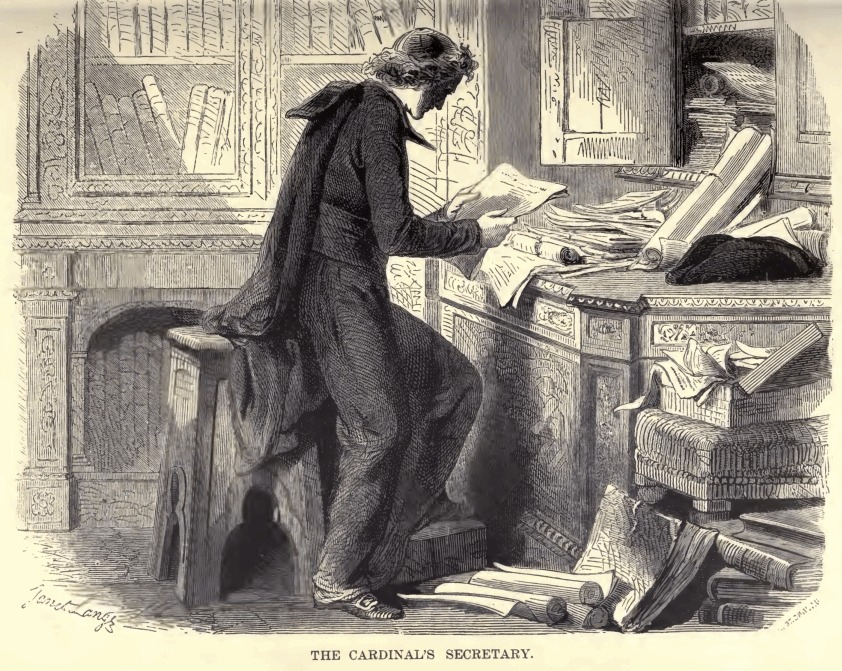
\includegraphics[width=\textwidth]{0245m.jpg}
\end{figure}

“This 25th day of April, 1498, be...ing invited to dine by his Holiness
Alexander VI., and fearing that not...content with making me pay for my
hat, he may desire to become my heir, and re...serves for me the fate
of Cardinals Caprara and Bentivoglio, who were poisoned,...I declare to
my nephew, Guido Spada, my sole heir, that I have bu...ried in a place
he knows and has visited with me, that is, in...the caves of the small
Island of Monte Cristo, all I poss...essed of ingots, gold, money,
jewels, diamonds, gems; that I alone...know of the existence of this
treasure, which may amount to nearly two mil...lions of Roman crowns,
and which he will find on raising the twentieth ro...ck from the small
creek to the east in a right line. Two open...ings have been made in
these caves; the treasure is in the furthest a...ngle in the second;
which treasure I bequeath and leave en...tire to him as my sole heir.
“25th April, 1498. “Cæs...ar † Spada.”

“Well, do you comprehend now?” inquired Faria.

“It is the declaration of Cardinal Spada, and the will so long sought
for,” replied Edmond, still incredulous.

“Yes; a thousand times, yes!”

“And who completed it as it now is?”

“I did. Aided by the remaining fragment, I guessed the rest; measuring
the length of the lines by those of the paper, and divining the hidden
meaning by means of what was in part revealed, as we are guided in a
cavern by the small ray of light above us.”

“And what did you do when you arrived at this conclusion?”

“I resolved to set out, and did set out at that very instant, carrying
with me the beginning of my great work, the unity of the Italian
kingdom; but for some time the imperial police (who at this period,
quite contrary to what Napoleon desired so soon as he had a son born to
him, wished for a partition of provinces) had their eyes on me; and my
hasty departure, the cause of which they were unable to guess, having
aroused their suspicions, I was arrested at the very moment I was
leaving Piombino.

“Now,” continued Faria, addressing Dantès with an almost paternal
expression, “now, my dear fellow, you know as much as I do myself. If
we ever escape together, half this treasure is yours; if I die here,
and you escape alone, the whole belongs to you.”

“But,” inquired Dantès hesitating, “has this treasure no more
legitimate possessor in the world than ourselves?”

“No, no, be easy on that score; the family is extinct. The last Count
of Spada, moreover, made me his heir, bequeathing to me this symbolic
breviary, he bequeathed to me all it contained; no, no, make your mind
satisfied on that point. If we lay hands on this fortune, we may enjoy
it without remorse.”

“And you say this treasure amounts to——”

“Two millions of Roman crowns; nearly thirteen millions of our money.”\footnote[2]{\$2,600,000
in 1894.}

“Impossible!” said Dantès, staggered at the enormous amount.

“Impossible? and why?” asked the old man. “The Spada family was one of
the oldest and most powerful families of the fifteenth century; and in
those times, when other opportunities for investment were wanting, such
accumulations of gold and jewels were by no means rare; there are at
this day Roman families perishing of hunger, though possessed of nearly
a million in diamonds and jewels, handed down by entail, and which they
cannot touch.”

Edmond thought he was in a dream—he wavered between incredulity and
joy.

“I have only kept this secret so long from you,” continued Faria, “that
I might test your character, and then surprise you. Had we escaped
before my attack of catalepsy, I should have conducted you to Monte
Cristo; now,” he added, with a sigh, “it is you who will conduct me
thither. Well, Dantès, you do not thank me?”

“This treasure belongs to you, my dear friend,” replied Dantès, “and to
you only. I have no right to it. I am no relation of yours.”

“You are my son, Dantès,” exclaimed the old man. “You are the child of
my captivity. My profession condemns me to celibacy. God has sent you
to me to console, at one and the same time, the man who could not be a
father, and the prisoner who could not get free.”

And Faria extended the arm of which alone the use remained to him to
the young man, who threw himself upon his neck and wept.
